\documentclass{beamer}
\usepackage[english]{babel}
\usepackage{ragged2e}   %justification

%\usetheme{Hannover}


% To print page number and footer
\setbeamertemplate{footline}[text line]{
  \parbox{\linewidth}{\vspace*{-8pt}Mr. Harish D. Gadade\hfill\insertshortauthor\hfill\insertpagenumber}}
\setbeamertemplate{navigation symbols}{}
\author[Govt. Colleg of Engg, Jalgaon]{}
% End Page number and footer

% To pring Header
%\setbeamertemplate{headline}{%
%\leavevmode%
 % \hbox{%
  %  \begin{beamercolorbox}[wd=\paperwidth,ht=2.5ex,dp=1.125ex]{palette quaternary}%
   % \insertsectionnavigationhorizontal{\paperwidth}{}{\hskip0pt plus1filll}
    %\end{beamercolorbox}%
 % }
%}
%End Header

% Logo do canto inferior direito
%\pgfdeclareimage[height=0.7cm]{gcoejLogo}{gcoejLogo}
\pgfdeclareimage[height=1cm]{gcoejLogo}{gcoejLogo}
\logo{
	\vspace*{8.2cm}
	%\vspace*{-0.25cm}
	\pgfuseimage{gcoejLogo}
	\hspace*{-0.05cm}}
	%\hspace*{-0.05cm}}


\begin{document}
\section{Message Passing}

\subsection{Introduction}
\begin{frame}
	\centering
	\large Unit-II\\
	\huge Message Passing\\
	\vspace{2cm}
	\small{Mr. Harish D. Gadade}\\
	\small{Govt. College of Engg., Jalgaon}
	
\end{frame}


\begin{frame}
	\frametitle{Introduction}
		Two basic methods for for information sharing as as follows
		\begin{enumerate}
		\item Shared Data Approach\\
		\begin{figure}
			\centering
			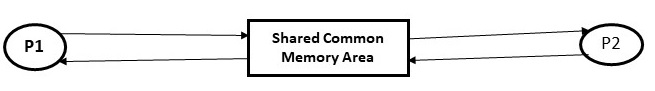
\includegraphics[width=8cm]{sharedDataApproach.jpg}\\
			\caption{Shared Data Approach}
		\end{figure}
		\item Message Passing Approach\\
		\begin{figure}
			\centering
			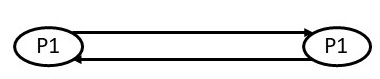
\includegraphics[width=7cm]{messagePassingApproach.jpg}
			\caption{Message Passing Approach}
		\end{figure}
		\end{enumerate}
\end{frame}

\subsection{Features of MPS}
\begin{frame}
	\frametitle{Desirable Features of a good Message Passing System}
	\begin{enumerate}
		\item \textit{Simplicity}
		\item \textit{Uniform Semantics}
		\begin{itemize}
			\item \textit{Local Communication}
			\item \textit{Remote Communication}
		\end{itemize}
		\item \textit{Efficiency}
		\item \textit{Reliability}
		\item \textit{Correctness}\\
			Issues related to correctness are
		\begin{itemize}
			\item \textit{Atomicity}
			\item \textit{Ordered Delivery}
			\item \textit{Survivability}
		\end{itemize}
		\item \textit{Flexibility}
		\item \textit{Security}
		\item \textit{Portability}
	\end{enumerate}
\end{frame}


\subsection{Issues}
\begin{frame}[allowframebreaks]
	\frametitle{Issues in IPC by Message Passing}
	\justifying{A message is a block of information formatted by a sending process in such a manner that it is meaningful to the receiving process.\\
	In the designing of an IPC protocol for message-passing system, the following important issues need to be considered.}
	\begin{figure}
		\centering
		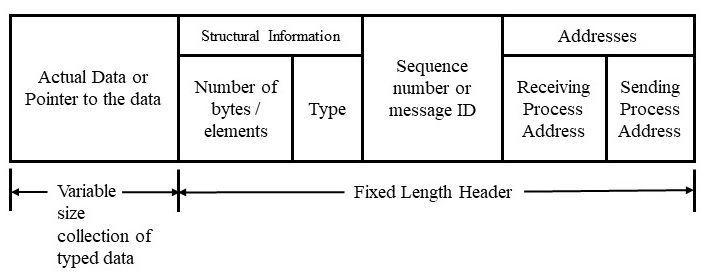
\includegraphics[width=10cm]{messageStructure.jpg}
		\caption{A Typical Message Structure}
	\end{figure}
	\framebreak
	In designing of an IPC for MPS, the following important issues need to be considered:
	\begin{enumerate}
		\item \textit{Who is the sender?}
		\item \textit{who is the receiver?}
		\item \textit{Is there one receiver or many receivers?}
		\item \textit{Is the message guaranted to have been accepted by its receiver?}
		\item \textit{Does the sender need to wait for a reply?}
		\item \textit{What should be done is a catastrophic event such as a node crash of a communication link failure occurs during the course of 
		communication?}
		\item \textit{What should be done if the receiver is not ready to accept the message:Will the message be discarded or stored in a buffer? In case 
		of buffering,what shoul be done if athe buffer is full?}
		\item \textit{Is there are several outstanding messages for a receiver, can it choose the order in which to service the outstanding messages?}
	\end{enumerate}	
\end{frame}


\subsection{Synchronization}
\begin{frame}[allowframebreaks]
	\frametitle{Synchronization}
	A central issue in the communication structure is the synchronization. The semantics
	used synchronization may be broadly classified as
	\begin{itemize}
		\item \textit{Blocking}
		\item \textit{Non-Blocking}
	\end{itemize}
	When both the send and receive primitives of a communication between two processes use
	blocking semantics, the communication is said to be synchronous; otherwise it is
	asynchronous.
	\vspace{2cm}
	\framebreak
	\begin{figure}
		\centering
		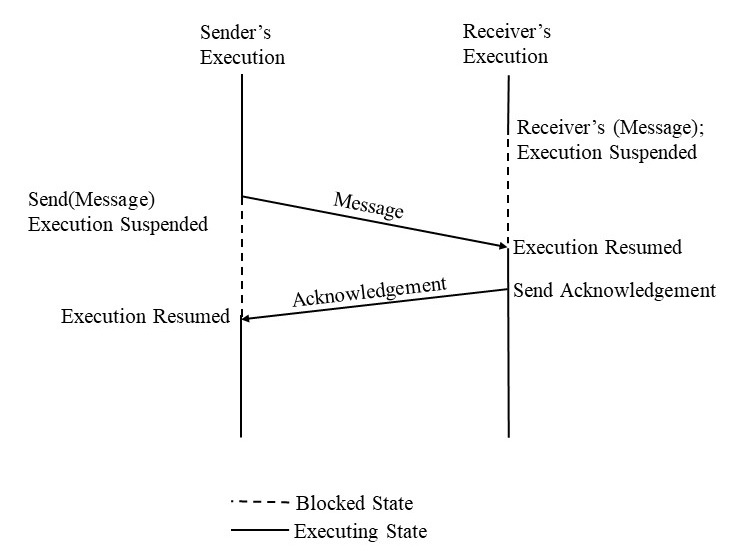
\includegraphics[width=9cm]{synchronousMode.jpg}
		\caption{Synchronous Mode of Communication with send and receive primitives having
		blocking type semantics.}
	\end{figure}
\end{frame}


\subsection{Buffering}
\begin{frame}[allowframebreaks]
	\frametitle{Buffering}
	The synchronous and asunchronous mode of communication correspond respectively to the
	two extremes of buffering: a Null Buffer or No Buffering and a buffer with unbounded
	capacity. Other two commonly used buffering strategies are Single-buffering and finite
	bound or multiple message buffers. These four types of buffering strategies are;
	\begin{itemize}
		\item \textit{Null Buffer or No Buffering}
		\item \textit{Single Message Buffer}
		\item \textit{Unbounded-Capacity Buffer}
		\item \textit{Finite Bound or Multiple Message Buffer}
	\end{itemize}
	\vspace{1.5cm}		
	\framebreak
	\begin{figure}
		\centering
		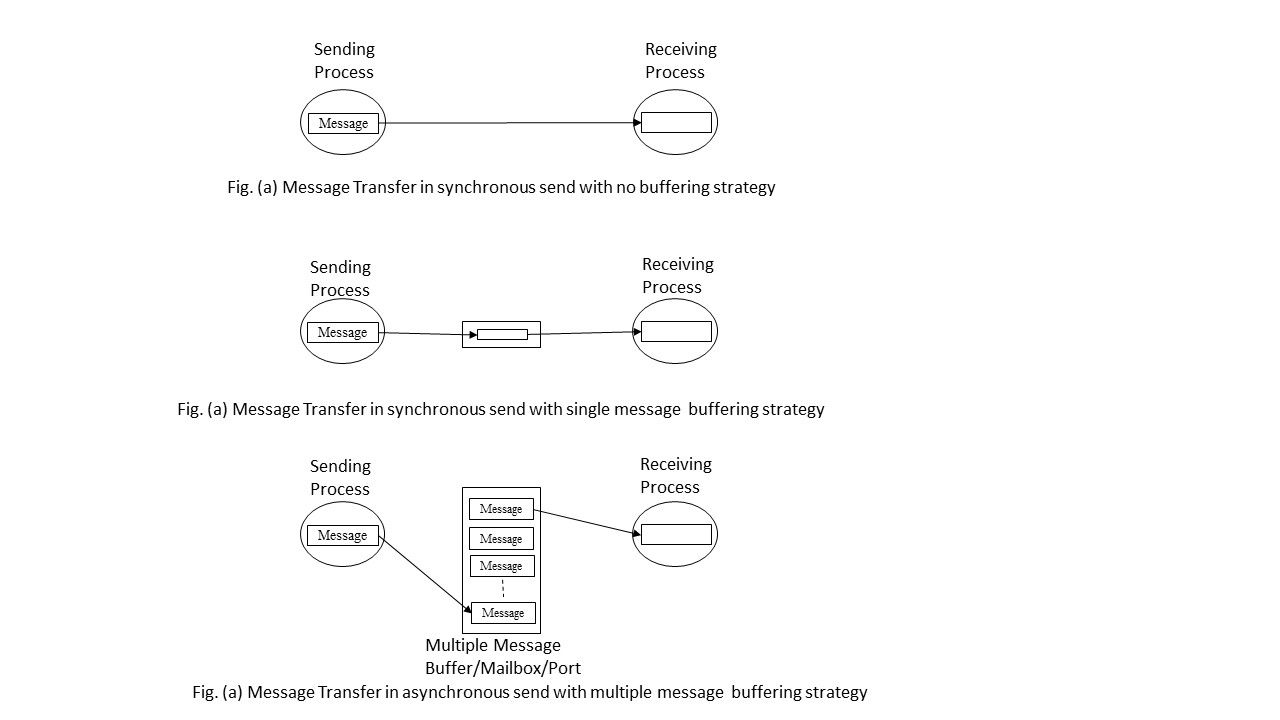
\includegraphics[width=15cm]{buffering.jpg}
	\end{figure}
	\vspace{1cm}
\end{frame}



\subsection{Multidatagram}
\begin{frame}
	\frametitle{Multidatagram Messages}
	\begin{itemize}
		\item \textit{Datagram}
		\item \textit{MTU}
		\item \textit{Single Datagram Messages}
		\item \textit{Multi Datagram Messages}
	\end{itemize}
	\vspace{4cm}
\end{frame}


\subsection{Encoding & Decoding}
\begin{frame}
	\frametitle{Encoding and Decoding of Message Data}
	\justifying{A message data should be meaningful to the receiving process. This implies that,
	ideally, the structure of the program object should be preserved while they are being
	transmitted from address space pf the sending process to the address space of the
	receiving process. This obviously is not possible in a heterogeneous systems in which
	the sending and receiving processes are on different computers of different
	architectures. However, even in homogeneous systems, it is very difficult to achieve
	this goal mainly because of two reasons:}
	\begin{enumerate}
		\item \textit{An absolute pointer value loses}
		\item \textit{Different program objects occupy varying amount of storage space.}
	\end{enumerate}
	Due to above mentioned problem encoding and decoding is done.\\
	One of the following two representations may be used for encoding and decoding of a message data.
	\begin{enumerate}
		\item \textit{In tagged representation}
		\item \textit{In Untagged representation}
	\end{enumerate}
\end{frame}


\subsection{Process Addressing}
\begin{frame}
	\frametitle{Process Addressing}
	Another important issue in message based communication is addressing(or naming)of the
	parties involved in an interaction.\\MPS usually supports two types of process
	addressing.
	\vspace{0.5cm}
	\begin{itemize}
		\item \textit{Explicit Addressing}
		\item \textit{Implicit Addressing}
	\end{itemize}
	\vspace{5cm}
\end{frame}


\subsection{Failure Handling}
\begin{frame}[allowframebreaks]
	\frametitle{ Failure Handling}
	While distributed system may offer potential for parallelism, it is also prone to
	partial failure such as node crash or a communication link failure. Therefore, during
	interprocess communication, such failures may lead the following problems:
	\begin{enumerate}
		\item \textit{Loss of Request Message}
		\item \textit{Loss of Response Message}
		\item \textit{Unsuccessful Execution of the Request}
	\end{enumerate}	
	\framebreak
	\begin{figure}
		\centering
		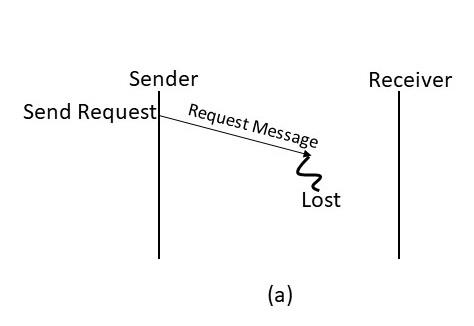
\includegraphics[width=10cm]{fig36(a).jpg}
		\caption{Request message is lost}
	\end{figure}
	\framebreak	
	\begin{figure}
		\centering
		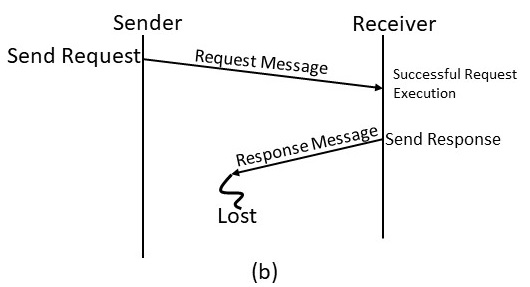
\includegraphics[width=10cm]{fig36(b).jpg}
		\caption{Response message is lost}
	\end{figure}
	\framebreak	
	\begin{figure}
		\centering
		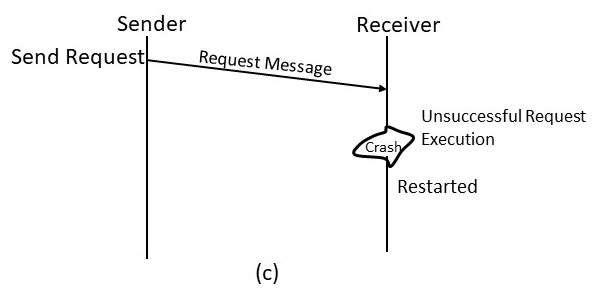
\includegraphics[width=10cm]{fig36(c).jpg}
		\caption{Receiver's computer crashed}
	\end{figure}
	\framebreak	
	To cope up with these problems, a reliable IPC protocol of a MPS is normally designed
	based on the idea of internal retransmission of message after timeouts and the return
	of the acknowledgement message of the sending machine's kernel be the receiving
	machine's kernel.\\Based on the above idea, a fourway message reliable IPC protocol
	for client-server between two processes works as follows:
	\begin{enumerate}
		\item \textit{Four-Message Reliable IPC Protocol}
		\item \textit{Three-Message Reliable IPC Protocol}
		\item \textit{Two-Message Reliable IPC Protocol}
	\end{enumerate}		
	\begin{figure}
		\centering
		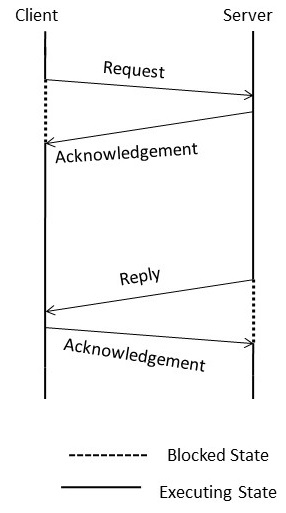
\includegraphics[width=4cm]{fig37.jpg}
		\caption{Four-message reliable IPC protocol}
	\end{figure}
\end{frame}

\begin{frame}
	\frametitle{Failure Handling(Continues...)}
	\begin{figure}
		\centering
		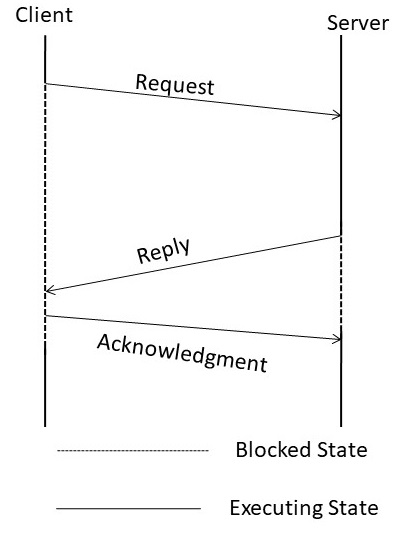
\includegraphics[width=4cm]{fig38.jpg}
		\caption{Three-message reliable IPC protocol}
	\end{figure}	
\end{frame}	

\begin{frame}
	\frametitle{Failure Handling(Continues...)}
	\begin{figure}
		\centering
		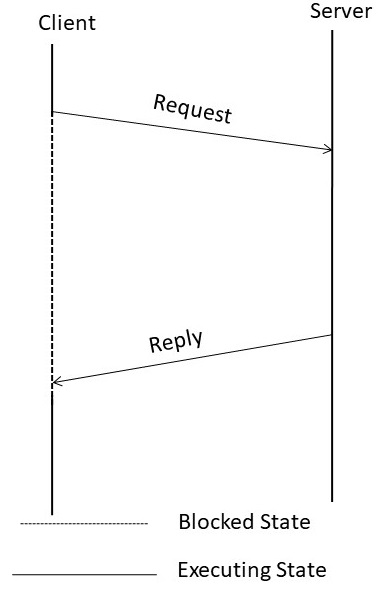
\includegraphics[width=4cm]{fig39.jpg}
		\caption{Two-message reliable IPC protocol}
	\end{figure}	
\end{frame}	


\begin{frame}
	\frametitle{Failure Handling(Continues...)}
	Consider an example of fault-tolerant communication between a client and a server
	\begin{figure}
		\centering
		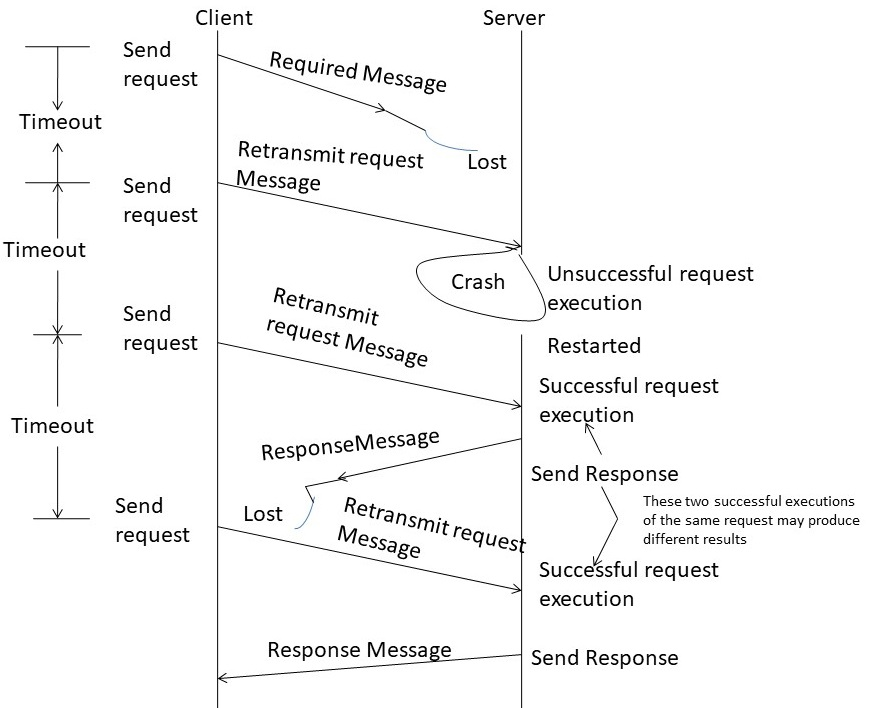
\includegraphics[width=8cm]{fig310.jpg}
		\caption{fault-tolerant communication between a client and a server}
	\end{figure}	
\end{frame}	


\subsubsection{Idem-potency}
\begin{frame}[allowframebreaks]
	\frametitle{Idem-potency and Handling of Duplicate Messages}
	
	\justifying{Consider the following routine of a server process that debits a specified amount from
	a bank and returns the balance amount to a requesting client.}
	%debit(amount)\\
	%if(balance>=amount)\\
	%{\\	
	%balance=balance-amount;\\
	%return("Success",balance)\\
	%else\\
	%return("Failure",balance)\\
	%end
	\begin{figure}
		\centering
		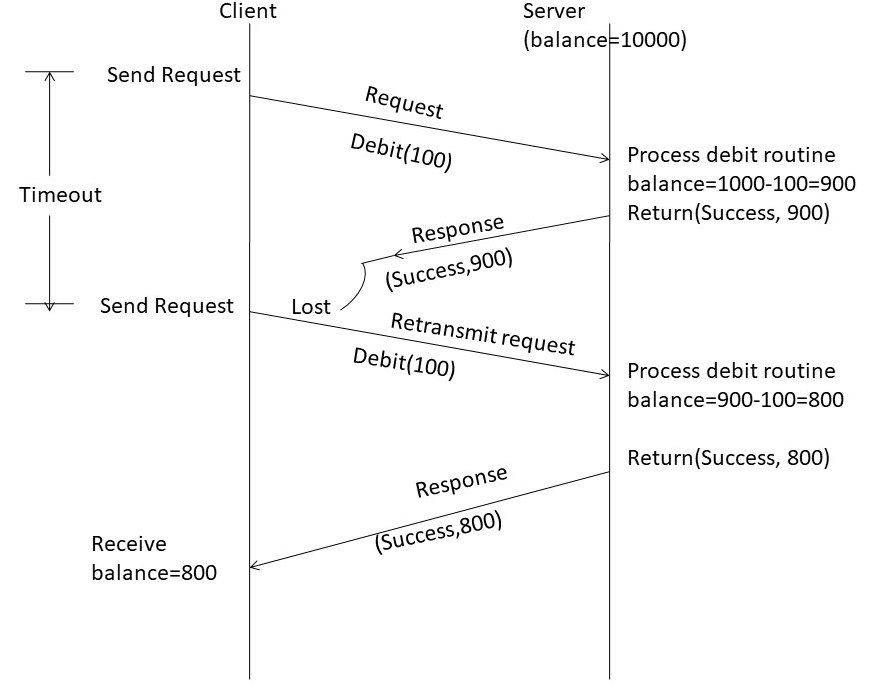
\includegraphics[width=6cm]{fig311.jpg}
		\caption{A Non-idempotent routine}
	\end{figure}
	\framebreak
	\begin{figure}
		\centering
		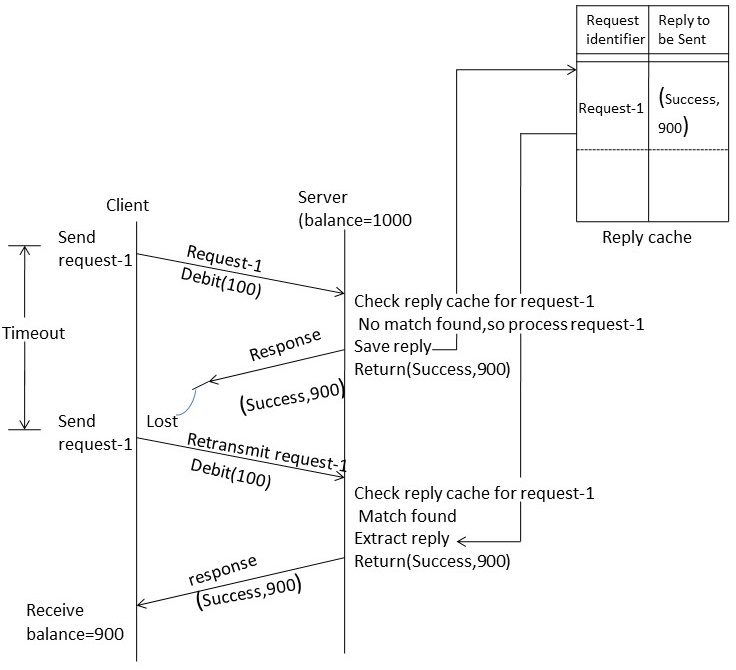
\includegraphics[width=8cm]{fig312.jpg}
		\caption{Exactly once semantics}
	\end{figure}
\end{frame}

\subsection{Group Communication}
\begin{frame}[allowframebreaks]
	\frametitle{Group Communication}
	Depending on single or multiple senders and receivers, the following are the three 
	types of group communications;
	\begin{enumerate}
		\item \textit{One-to-Many}
		\item \textit{Many-to-One}
		\item \textit{Many-to-Many}
	\end{enumerate}	
	\vspace{4cm}
	\framebreak
	1. One-to-Many
	\begin{itemize}
				\item \textit{Group Management}
				\item \textit{Group Addressing}
				\item \textit{Message Delivery to Receiver Process}
				\item \textit{Buffered and Unbuffered Multicast}
				\item \textit{Send-to-All and Bulletin-Board Semantics}
				\item \textit{Flexible Reliability in Multicast Communication}
				\item \textit{Atomic Multicast}
				\item \textit{Group Communication Primitives}
		\end{itemize}
		\vspace{2cm}
\end{frame}
\end{document} 